\section{Problem Statement}
\label{sec:problem-statement}
Let $T^s \in SE(3)$ be the initial 6D pose of a unknown 3D rigid object $O$ in the world coordinate frame, consisting of a rotation $R^s \in SO(3)$ and a translation $t^s \in \mathbb{R}^3$. Given $O$ with starting pose $T^s$ and a kitting cavity $K$, let $\mathcal{G} \subset SE(3)$ be the set of goal 6-DOF poses of object $O$ that result in successful kitting. The goal is to orient object $O$ to $T^g \in \mathcal{G}$, where $T^g$ consists of rotation $R^g$ and translation $t^g$. Figure~\ref{fig:mug-cavity-2} shows a simulated example where a 3D object $O$ is successfully kitted into a concave cavity $K$.
% \MD{Note about range of rotations that cause the object to kit correctly? This is implied by G but not stated explicitly anywhere. I think we need to formalize this a bit more.} \SD{We wanted some sim trials on object cavity pairs for this, but we don't have time to formalize that by March 15 because creating the cavities is pretty tough, and then we would have to setup the pybullet environment}.

\subsection{Assumptions}
\label{subsec:formulation}
We assume access to depth images of a rigid object $O$ and a kitting cavity $K$. The cavity image may be taken with the cavity either in its standard, concave orientation (i.e., open to object insertion), or flipped, convex orientation (i.e., mirroring the shape of the object to be inserted).
% We also assume that the rotation angle between $R^s$ and $R^g$ is at most 30\degree \SD{Can we say 45 degrees or 60 degrees? It can be 60 degrees away from a correct orientation, but still be 30 degrees from the set of correct orientations}. 
We also assume that orienting $O$ to a pose in $T^g \in G$ and releasing the gripper results in a successful kitting action.

\begin{figure}[t]
  \centering
  \vspace{8pt}
  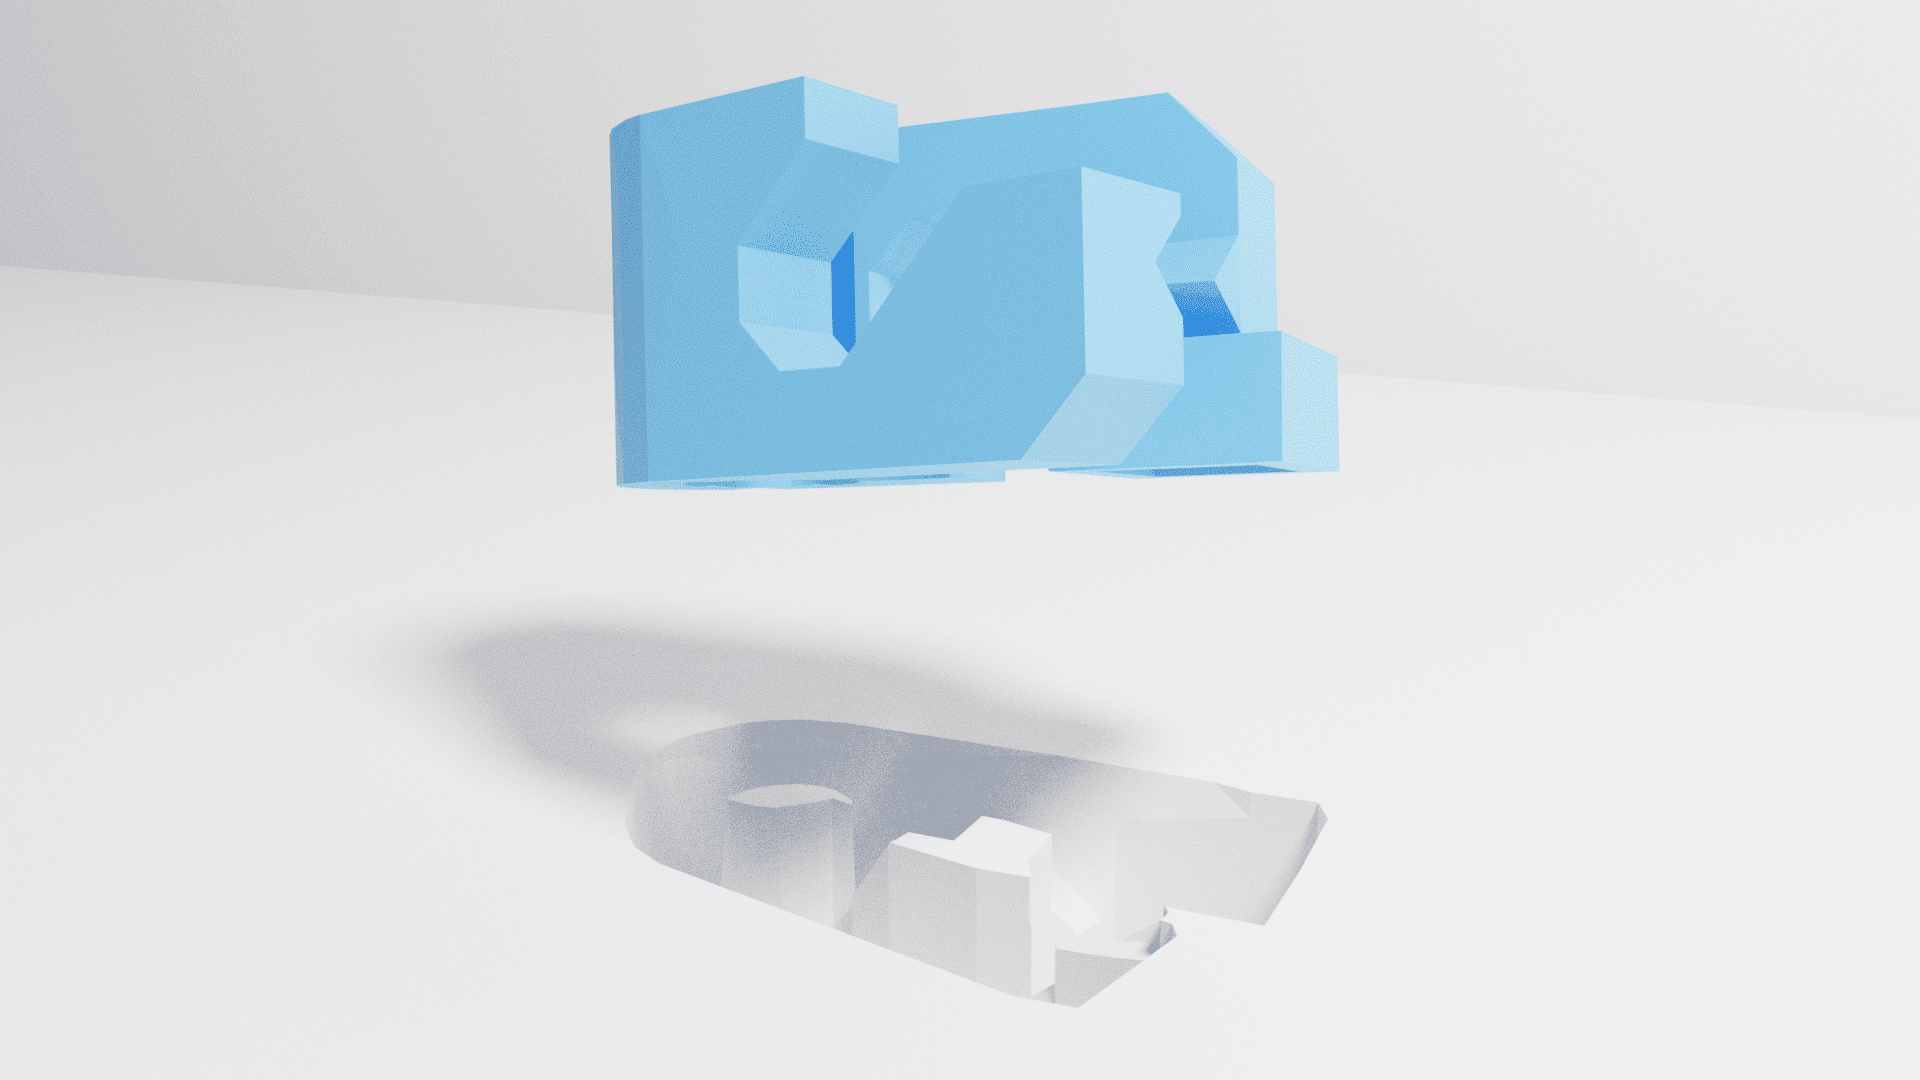
\includegraphics[width=121pt,trim=440 0 440 0, clip]{figures/bar_clamp_impression_2.png}\hfill%
  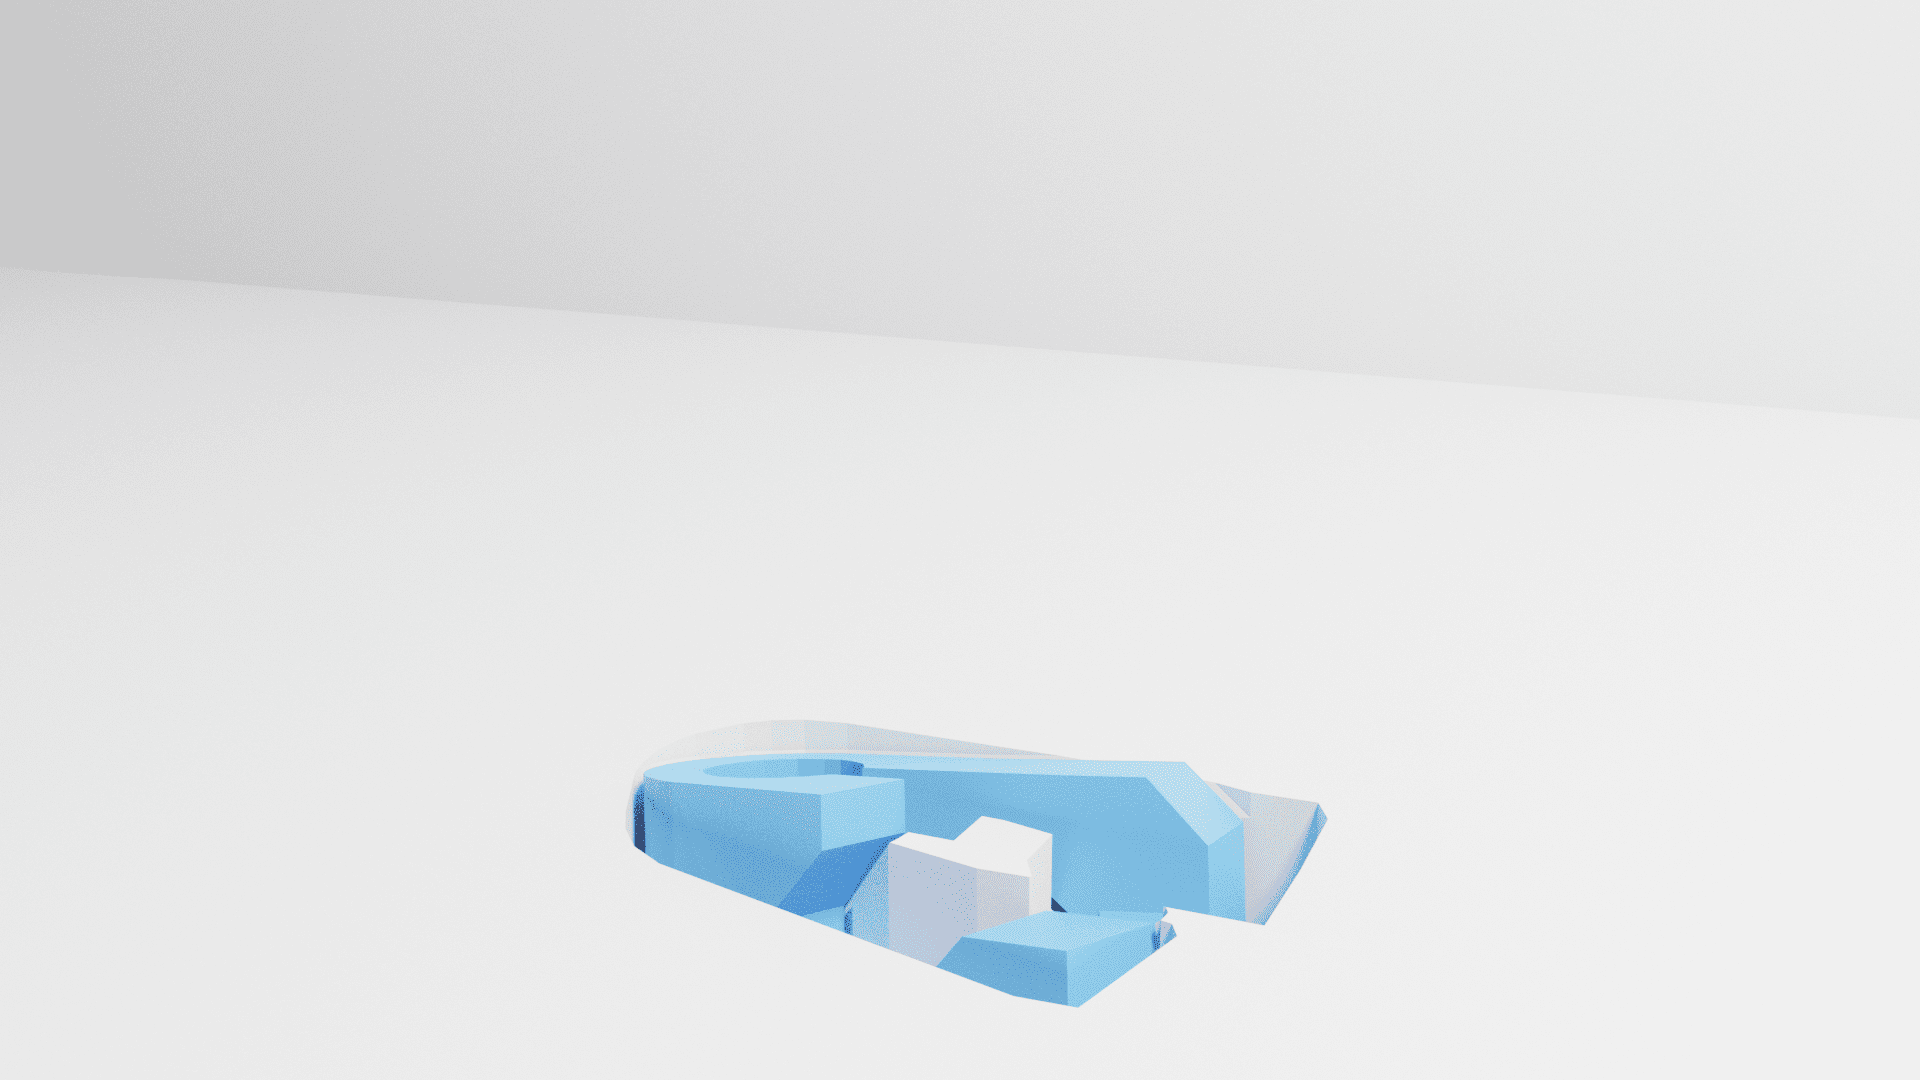
\includegraphics[width=121pt,trim=440 0 440 0, clip]{figures/bar_clamp_impression_4.png}
  \caption{\textbf{Successful Kitting: }Visualization of successfully kitting a 3D object into a concave cavity.}
  %\caption{\textbf{Generating Negative Goal Images: }Example an object (left) in a specific configuration $T^g$ and its complementary cavity created in simulation with Blender. We use the fatten operation to create a cavity with some slack for insertion (right). 
%   This cavity requires orienting the object to $\mathcal{G}$, a range of poses close to $T^g$ in order to be oriented.
  %}
  \label{fig:mug-cavity-2}
\end{figure}
\subsection{Input}
\label{subsec:input}
Let $I^s \in \mathbb{R}^{H \times W}$ be a depth image observation of the object in initial pose $T^s$, and
$I^k \in \mathbb{R}^{H \times W}$ be the depth image observation of a kitting cavity, $K$. See Figure~\ref{fig:clamshell-cavities} for physical examples of objects and kitting cavities.

\subsection{Output}
\label{subsec:output}
%As shown in Fig.~\ref{fig:splash} and Fig.~\ref{fig:mug-cavity-2},
The goal is to successfully kit an unknown 3D object $O$ into a novel 3D cavity $K$ (Fig.~\ref{fig:splash}, Fig.~\ref{fig:mug-cavity-2}). Thus, we aim to transform the initial pose $T^s$ into a goal pose that fits into the cavity (i.e., $T^g \in \mathcal{G}$). For objects with symmetries, the objective is to estimate and orient objects relative to a (symmetric) orientation that results in successful insertion into the cavity K.

% \subsection{Background}
% We use unit quaternions to represent rotations.
% A quaternion $q = q_r + q_i i + q_j j + q_k k$ is an extension of complex numbers with a real component $q_r$ and 3 scaled fundamental imaginary units $i$, $j$, and $k$.
% We represent $q$ using the convention of a vector $\begin{bmatrix} q_r & q_i & q_j & q_k \end{bmatrix}^T$. 
% A \emph{unit} quaternion has the property that $\lVert q \rVert^2 = q_r^2 + q_i^2 + q_j^2 + q_k^2 = 1$, and can represent a rotation with properties we make use of in this work:
% \begin{description}[left=0pt]
%     \item[Normalization] A unnormalized or non-unit quaternion $\tilde{q}$ can be converted to a unit quaternion by dividing by its norm $\tilde{q} / \lVert \tilde{q} \rVert_2$
%     \item[Angle difference] The angle of rotation $\theta$ between two quaternions $q_0$ and $q_1$ is $2\cos^{-1} \lvert \langle q_0, q_1 \rangle \rvert$
%     \item[Rotation difference] The quaternion rotation between two quaternions is $q_{\mathrm{diff}} = q_0 q_1^{-1}$, where $q_1^{-1}$ is the conjugate (negated imaginary components) of $q_1$
%     \item[Slerp] The spherical linear interpolation or \emph{slerp} between rotations $q_0$ and $q_1$ by a scalar $t \in [0,1]$ is  $\Slerp(q_0, q_1, t) = (q_0 \sin (1-t)\theta + q_1 \sin t\theta) / \sin \theta$, where $\theta$ is the angle between the two rotations~\cite{shoemake}.
%     \item[Angle of rotation] The angle of rotation of a quaternion is defined by $\quattoangle(q) = 2 \cos^{-1} q_r$
%     \item[Axis of rotation] The axis of rotation of a quaternion is $\begin{bmatrix} q_i & q_j & q_k \end{bmatrix} / \sqrt{1 - q_r^2}$
%     \item[Double Coverage] Quaternions double cover $SO(3)$, in that $q$ and $-q$ represent the same rotation.
% \end{description}
